
\iffalse
\section*{ICES Background}

Observational data are imperfect, and predictive models based on those data represent simplifications of how some aspect of the world works. Thus, in the fisheries advisory process (e.g., development of catch advice using stock assessments, evaluation of management strategies), it is clear that our analyses are fraught with uncertainty, stemming from uncertainty in the input data (observations) or from the \laurie{structure (degree of simplification and validity of assumptions)} of the methods and models employed. Input uncertainty is easier to measure using standard statistical procedures, and to address through improvements to survey designs, sampling schemes, and statistical methods. \laurie{Structural uncertainties however, are more intangible as they often represent “known unknowns” - i.e., we know there are limitations to the methods and models, but it is difficult to describe and measure them without comprehensive analyses, such as simulation testing or cross-validation}.

With the development of more advanced analytical frameworks that support implementation of  machine learning, artificial intelligence, and ensemble modeling, we invite fisheries scientists to a session to present advances in \laurie{identifying, quantifying and dealing with structural uncertainties in the fisheries science advisory process.}

We invite contributions on the following themes:

\begin{itemize}
    \item \laurie{Uncertainties throughout the stock assessment and management strategy evaluation process}
    \item \laurie{Identification and testing of plausible structural hypotheses, and structural uncertainties}
    \item \laurie{Sensitivity analysis}
    \item \laurie{Model ensembles (within and between models) see previous \href{ https://www.fisheries.noaa.gov/national/population-assessments/noaa-fisheries-13th-national-stock-assessment-workshop-report-released}{NOAA workshop} }
    \item \laurie{Gaps and needs for developing ensembles}
    \item \laurie{Evaluating trade-offs between one versus multiple models}
    \item \laurie{Combining and communicating results across ensemble members and stakeholders}
\end{itemize}

\maketitle

\begin{abstract}
\end{abstract}
\fi

\maketitle


\begin{itemize}
    \item The adoption of the Precautionary Approach to fisheries management \citep[PA,][]{garcia1996precautionary} requires a formal consideration of uncertainty. In the stock assessment process uncertainty about resource dynamics are commonly represented by alternative model structure, datasets and parameters. 
    
    \item The use of integrated assessment models has meant that fitting to all available data has become commonplace as scientists seek to use the models to capture all knowledge about stock size and productivity \citep{hilborn2003state}. 
    
    \item %There has also been a trend in stock assessment toward the use of integrated analysis that combines several sources of data into a single model by a joint likelihood  \citep[e.g.][]{doubleday1976least,fournier1982general,maunder2013review}. 
    Problems remain, however, including a lack of information on processes such as density dependence, non-stationarity and conflicts between datasets. 
    
    \item Therefore, ensembles are often implemented with scenarios for hard to estimate parameters, such as natural mortality and the steepness of the stock recruitment relationship, and to explore data weighting.  
    
    \item Key questions are is my model valid? and do I have sufficient data and knowledge to fit it?  We therefore used hindcasting to estimate prediction skill as a tool for validation and weighting of scenarios. 
    
    \item The performance of multimodel ensembles depends on the weights given to the different models of the ensemble when post processing. This paper compares equal weighting of models (EW) to simple skill-based weighting (SW), using Mohn's $\rho$ as simple model performance indicator.
    
\end{itemize}

\newpage
\section*{Case Study}

\begin{figure}[ht!]\centering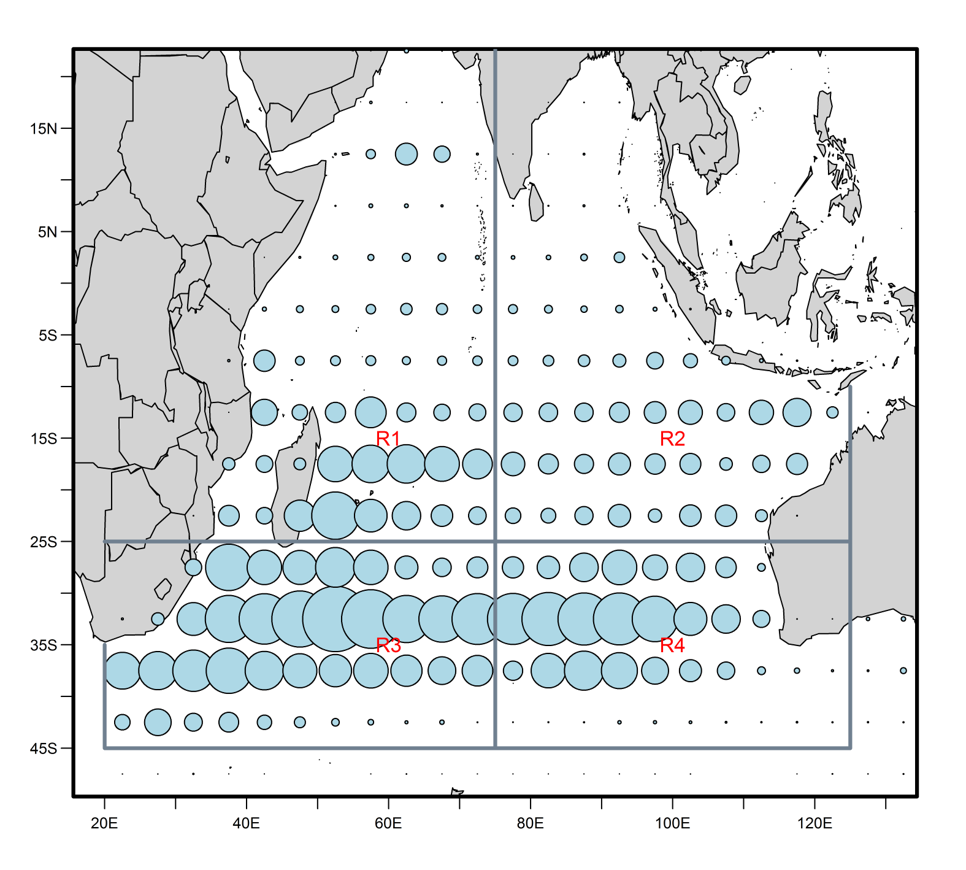
\includegraphics[width=0.75\textwidth]{figures/alb-map.png} 
\caption{Distribution of Indian Ocean albacore tuna catches by assessment areas.}
\label{fig:map}
\end{figure}

For Indian Ocean albacore, 1440 SS3 stock assessments were explored by fixing parameters (e.g. M, h, selection pattern) and data weighting. 


\begin{table}[ht]
\label{tab:grid}
\caption{Operating Model Scenarios; Base Case values in bold.}  
\begin{center}
\label{tab:datasumm}
\small

\begin{tabular}{|lccc|}

\hline
Factor & {Levels (N)} & {$\prod$ N} & {Values} \\ %& {Prior} & {Weighting}\\
\hline\hline
{Natural mortality (M)& {5}}  & {  5}  & { 0202  \textbf{0303} 0404 0403 0402}    \\
{Steepness of the stock-recruitment relationship}}& {3} 	 & {15}  & { \textbf{.7}; 0.8; 0.9} \\
{Variability of recruitment (sigmaR)}& {2} 	 & { 30}  & { \textbf{0.4}; 0.6} \\
{Effective Sampling Size of the length composition data (ESS)}& {3} & { 90}  & { 20; \textbf{50}; 100} \\
{CV for fit to CPUE (cpuecv)}& {2} 	 & { 360}  & { 0.2;  \textbf{0.3}; 0.4; 0.5} \\
{Yearly increase in catchability coefficient of CPUE (llq)}& {2} 	 & {  720}  & { \textbf{0\%}; 0.25\%} \\
  {Selectivity (llsel)}& {2}}& {1440}} & { \textbf{logistic} double normal} \\
\hline

\end{tabular}
\end{center}
\end{table}

\newpage
\section*{Methods}
\begin{itemize}
    \item Difficult to select models using metrics such as AIC. 
    \item Retrospective analysis is commonly used to evaluate the stability of stock assessment estimates of model estimates such as stock biomass and exploitation level. Stability is measured using Mohn's $\rho$ a measure of bias. 
    \item Shrinking estimates of stock status in the last year to the recent mean can help reduce Mohn's $\rho$. Shrinkage, in statistics, however, is used to reduce mean squared error (MSE), at the expense of bias. 
    \item The use of model based quantities, however, means that bias can not be quantified, and may result in future predictions being being poor. We therefore extend retrospective analyses to include prediction. 
\end{itemize}

\newpage
\newpage
\section*{Figures}

\begin{figure}[ht!]\centering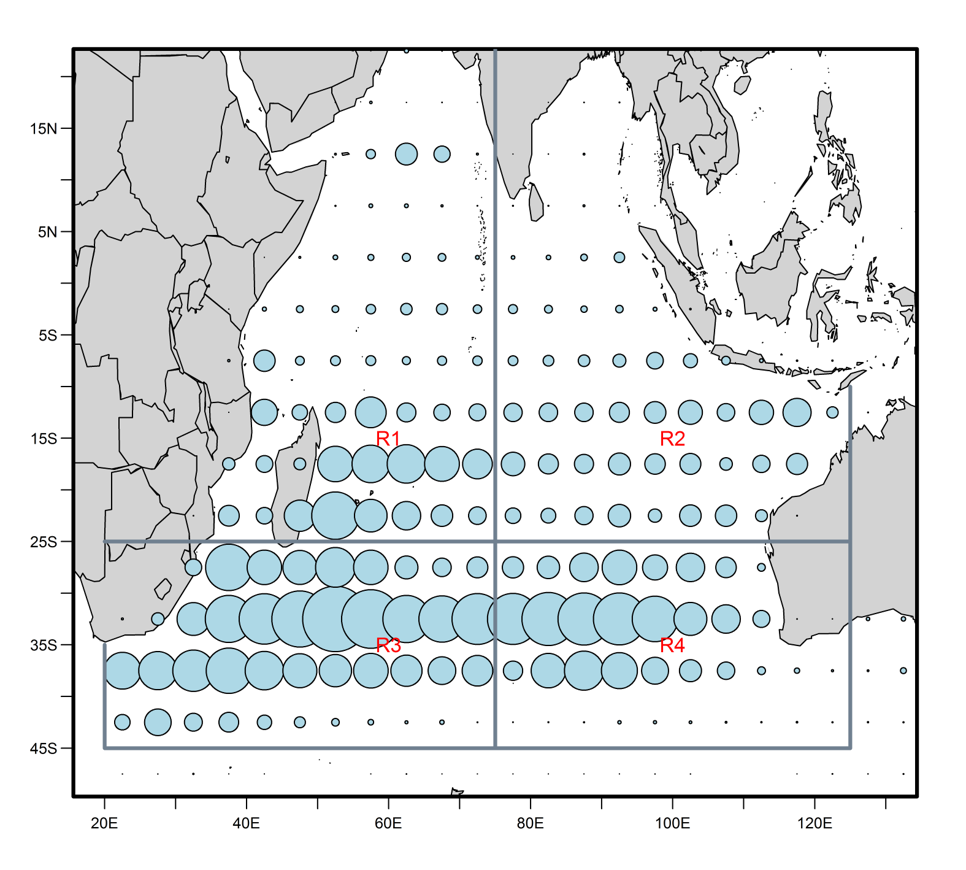
\includegraphics[width=0.75\textwidth]{figures/alb-map.png} 
\caption{Distribution of Indian Ocean albacore tuna catches by assessment areas.}
\label{fig:map}
\end{figure}

\begin{figure}[ht!]\centering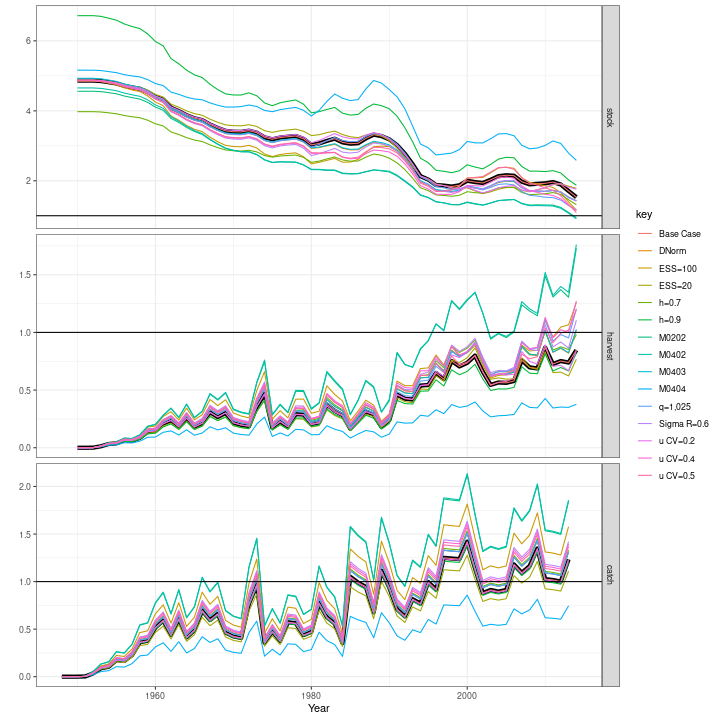
\includegraphics[width=0.75\textwidth]{figures/main-trends-1.png} \caption{Time series of spawning stock biomass and fishing mortality relative to $MSY$ target reference points for the main effects of the Indian Ocean albacore tuna assessment model grid.}
\label{fig:ts}
\end{figure}

\begin{figure}[ht!]\centering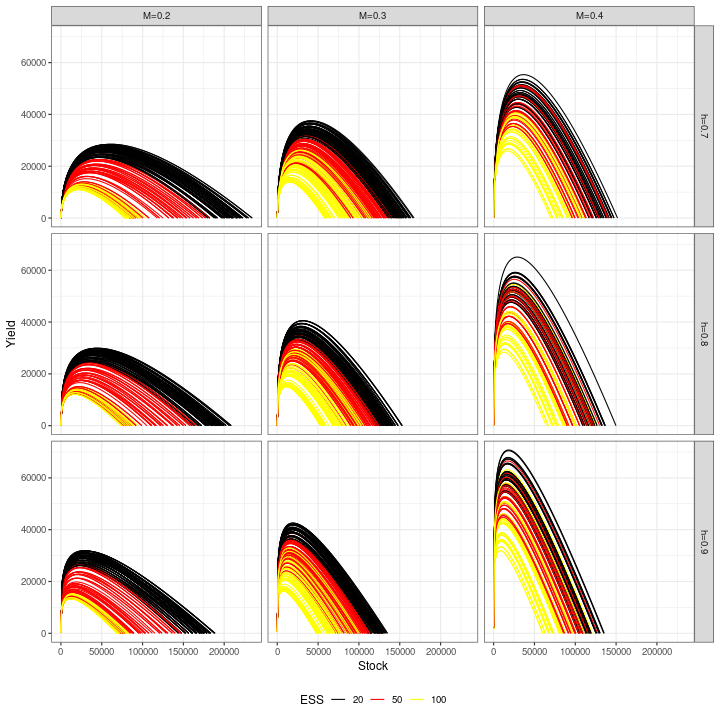
\includegraphics[width=0.75\textwidth]{figures/pf-grid-1.png} 
\caption{Production by steepness and mature natural mortality}
\label{fig:pf}       
\end{figure}

\begin{figure}
        \begin{subfigure}[b]{0.5\textwidth}
               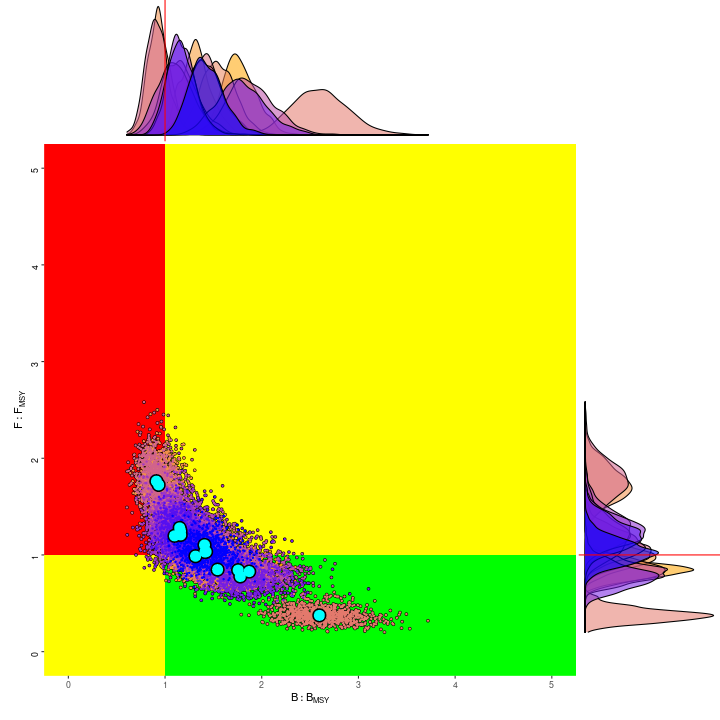
\includegraphics[width=\linewidth]{figures/kobe-main-1.png}
                \caption{Main effects with estimation error.}
                \label{fig:kobe-main}
        \end{subfigure}%
                \begin{subfigure}[b]{0.5\textwidth}
                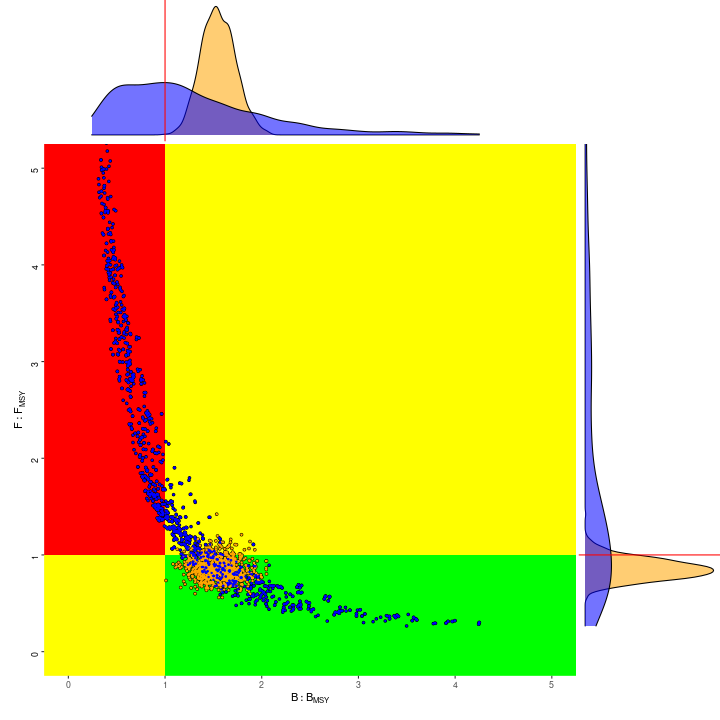
\includegraphics[width=\linewidth]{figures/kobe-bg-1.png}
                \caption{Reference case and grid with model.}
                \label{fig:kobe-bg}
        \end{subfigure}%
        \caption{Kobe phase plots showing spawning biomass ($B$) and fishing mortality ($F$) relative to $MSY$ target reference points. Within model uncertainty was approximating using multivariate log-normal distribution derived from Hessian matrix (MVLN) with cyan points denoting the median}\label{fig:kobe}
\end{figure}

\clearpage
\newpage
\begin{figure}[ht!]\centering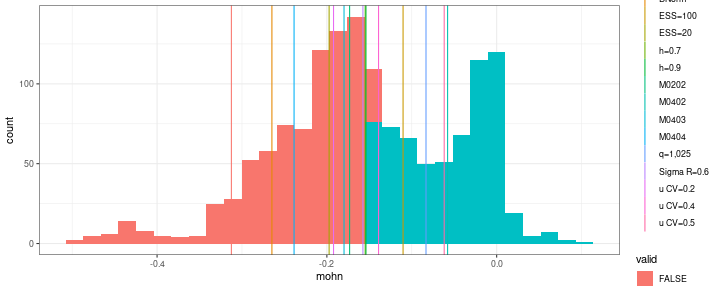
\includegraphics[width=0.75\textwidth]{figures/mohn3-1.png}  \caption{Summary of Mohn's $\rho$ for the for the 1440 assessment models in the Indian Ocean albacore tuna grid, with main effects indicated by the vertical lines.} 
\label{fig:mohn}       
\end{figure}

\begin{figure}
    \begin{subfigure}[a]{0.35\textwidth}
    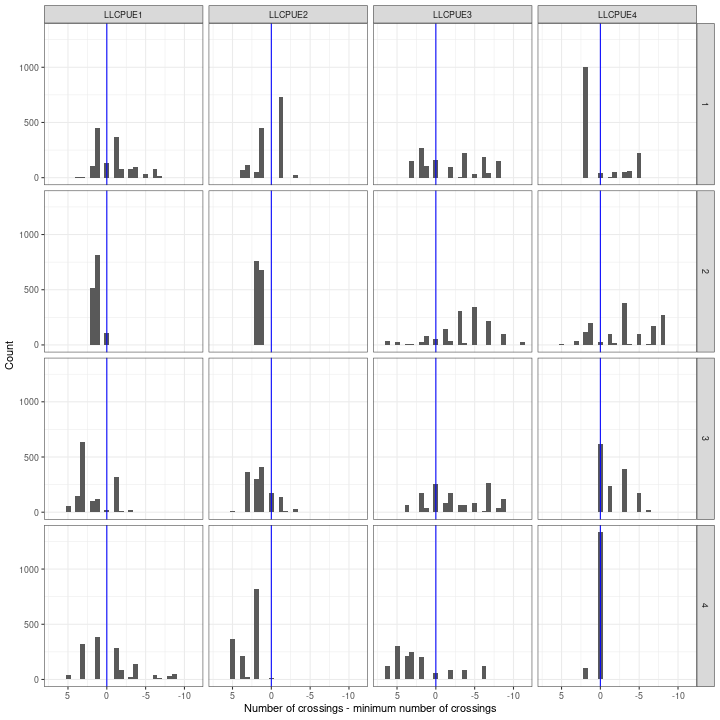
\includegraphics[width=\linewidth]{figures/run-cross-1.png}
    \caption{Number of crossings - minimum expected number of crossings; note reversed x-axis.}
    \label{fig:runs-cross} 
    \end{subfigure}%
    \begin{subfigure}[b]{0.35\textwidth}
    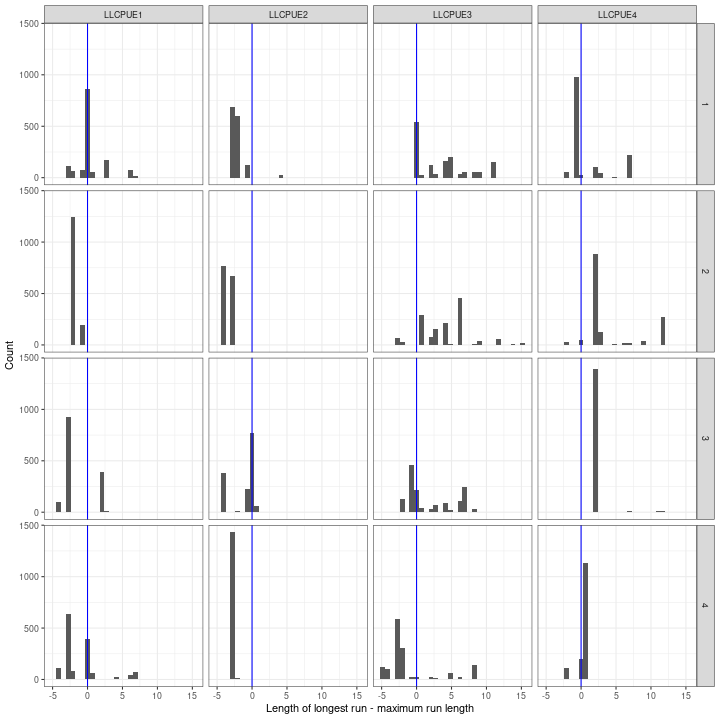
\includegraphics[width=\linewidth]{figures/run-long-1.png}
    \caption{Longest run - maximum expected run length.}
    \label{fig:runs-long}
    \end{subfigure}%
    \begin{subfigure}[c]{0.35\textwidth}
    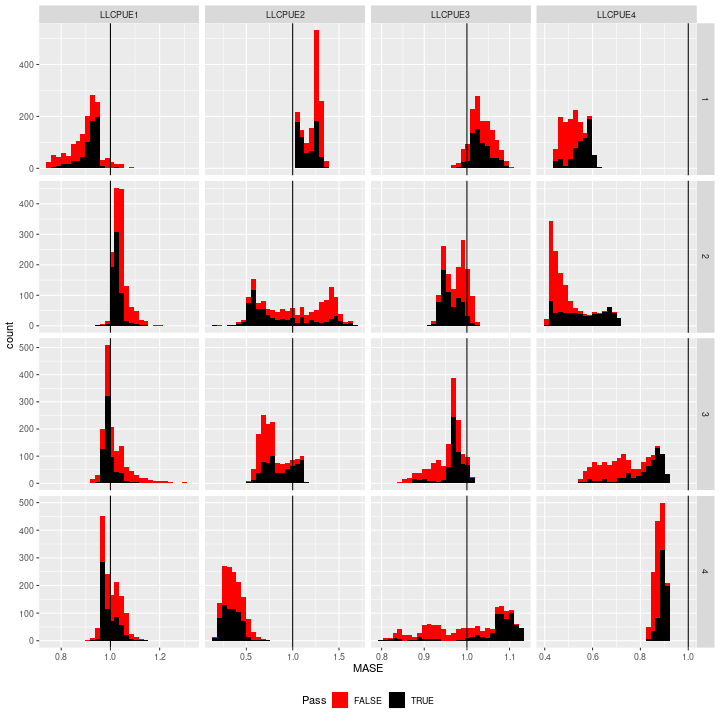
\includegraphics[width=\linewidth]{figures/mase-1.png}
    \caption{MASE.}
    \label{fig:mase}
    \end{subfigure}%
 
\caption{}\label{fig:runs}
\end{figure}


%\begin{figure}[ht!]\centering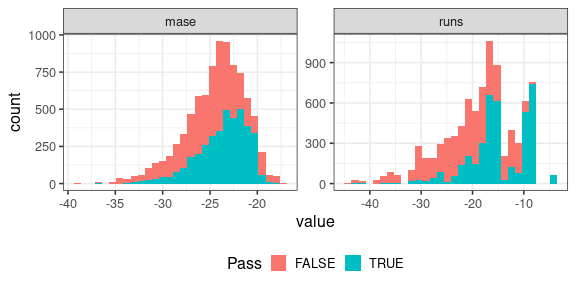
\includegraphics[width=0.75\textwidth]{figures/cf-1.png} \caption{Summary of weighting diagnostics.}\label{fig:wts} \end{figure}

\begin{figure}[ht!]\centering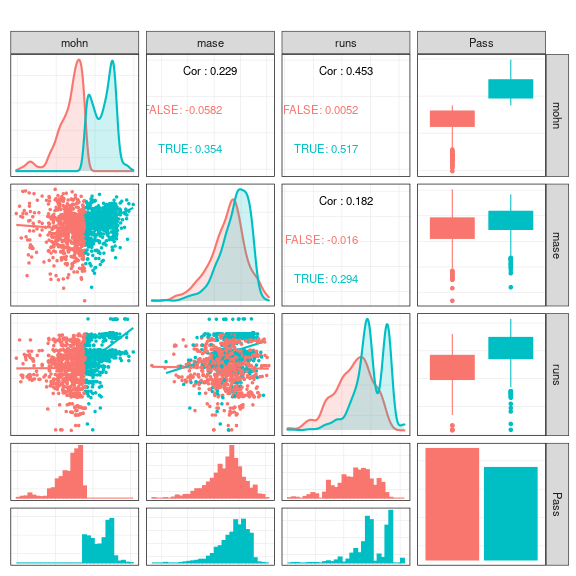
\includegraphics[width=0.75\textwidth]{figures/ggpair-1.png} \caption{Correlations between weighting diagnostics.}
\label{fig:wts}       
\end{figure}

\newpage
\begin{figure}[!ht]
	\centering
	\begin{subfigure}{0.9\textwidth}
		\centering
		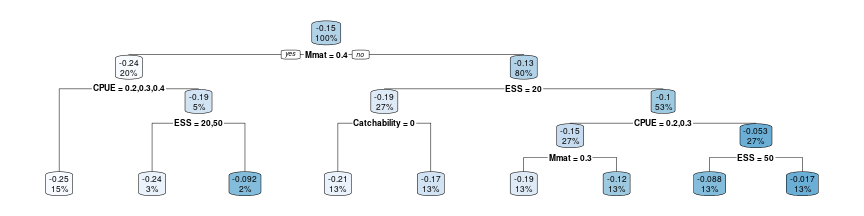
\includegraphics[width=\textwidth]{figures/a-tree-1.png}
		\caption{Regression Tree}
		\label{fig:tree}
	\end{subfigure}
	\hfill
	\begin{subfigure}{0.9\textwidth}  
		\centering 
		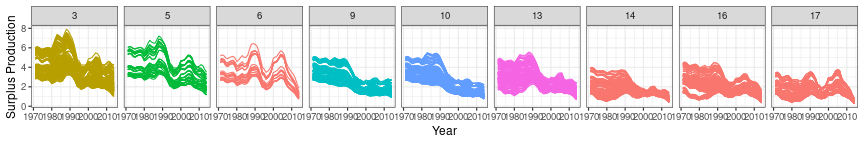
\includegraphics[width=\textwidth]{figures/a-tree-biomass-1.png}
		\caption{SSB}
		\label{fig:tree-b}
	\end{subfigure}
	\begin{subfigure}{0.9\textwidth}  
		\centering 
		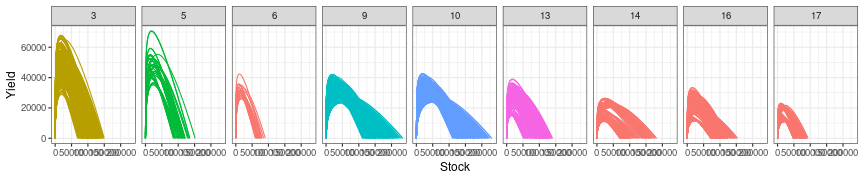
\includegraphics[width=\textwidth]{figures/a-tree-pf-1.png}
		\caption{Production Function}
		\label{fig:tree-pf}
	\end{subfigure}
	\begin{subfigure}{0.9\textwidth}
		\centering
	    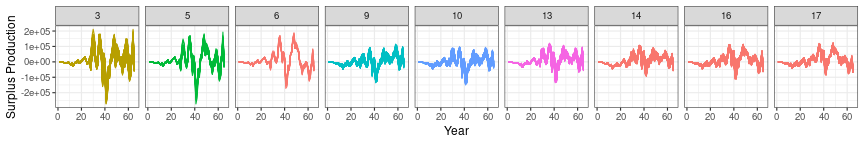
\includegraphics[width=\textwidth]{figures/a-tree-sp-1.png}
		\caption{Surplus Production}
		\label{fig:tree-sp}
	\end{subfigure}
	\caption{Mohn's $\rho$}
	\label{fig:tree}
\end{figure}


\begin{figure}
        \begin{subfigure}[b]{0.5\textwidth}
                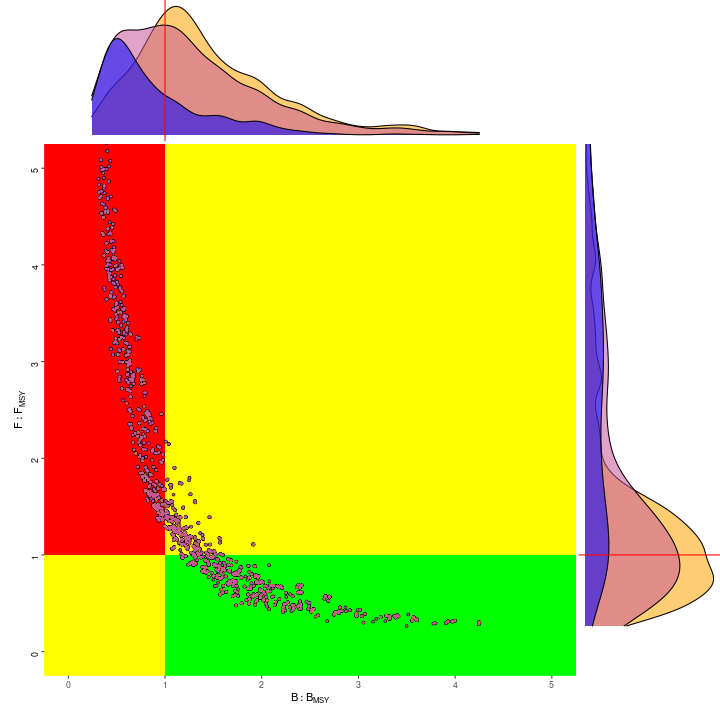
\includegraphics[width=\linewidth]{figures/kobe-mohn3-2.png}
                \caption{Kobe}
                \label{fig:kobe-wt}
        \end{subfigure}%
        \begin{subfigure}[b]{0.5\textwidth}
                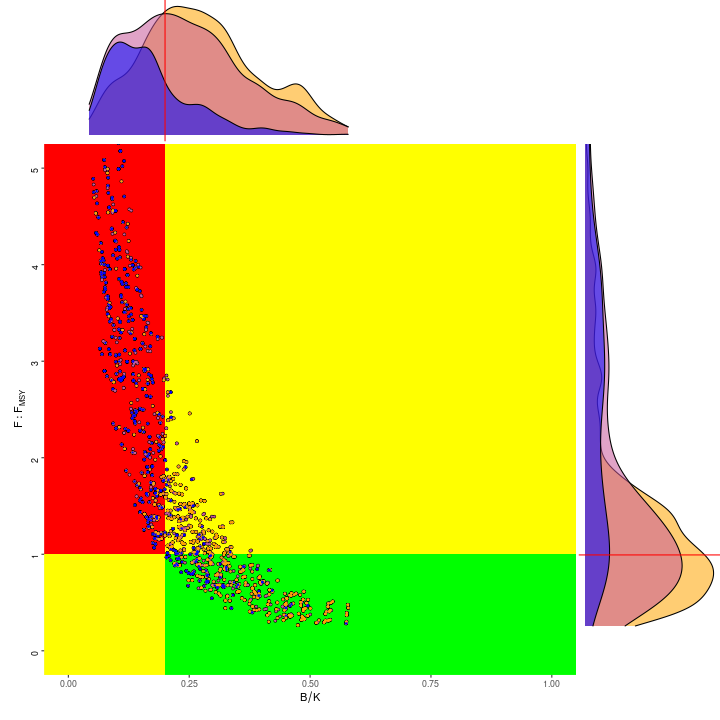
\includegraphics[width=\linewidth]{figures/majuro-mohn3-all-1.png}
                \caption{Majuro}
                \label{fig:majuro-wt}
        \end{subfigure}%
        \caption{Phase plots for all 1440 grid models, with equal, AIC, and skill weighting identifying models that pass the Mohn's $\rho$ test for hindcasts with 3 year ahead forecasts .}
        \label{fig:phase-wt}
\end{figure}


%\begin{figure}[ht!]\centering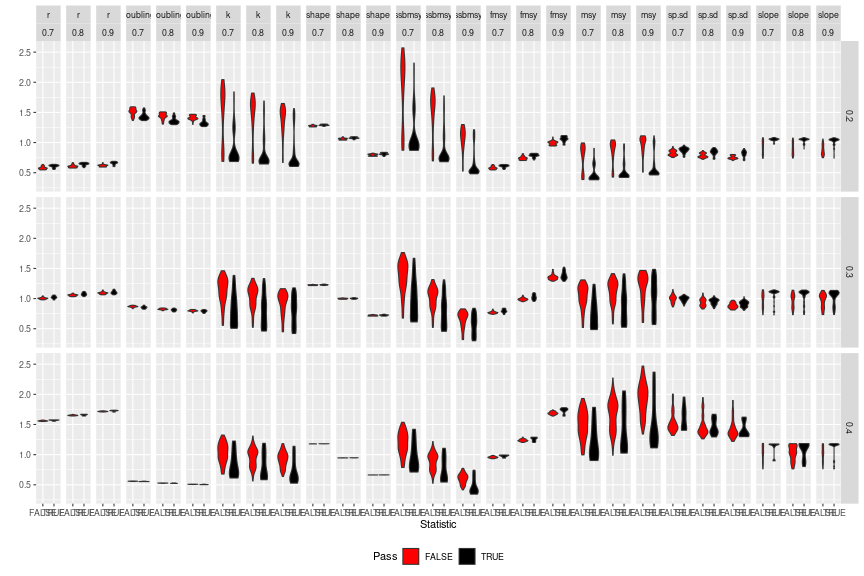
\includegraphics[width=1\textwidth]{figures/param-box-mohn3-1.png}\caption{Summary statistics, will re-do for $F/F_{MSY}$, $B/B_{MSY}$, $r$, $K$, $p$ and $sd(sp)$, and population doubling time.}\label{fig:smry}\end{figure}

\newpage
\begin{figure}[!ht]
	\centering
	\begin{subfigure}{0.32\textwidth}
		\centering
		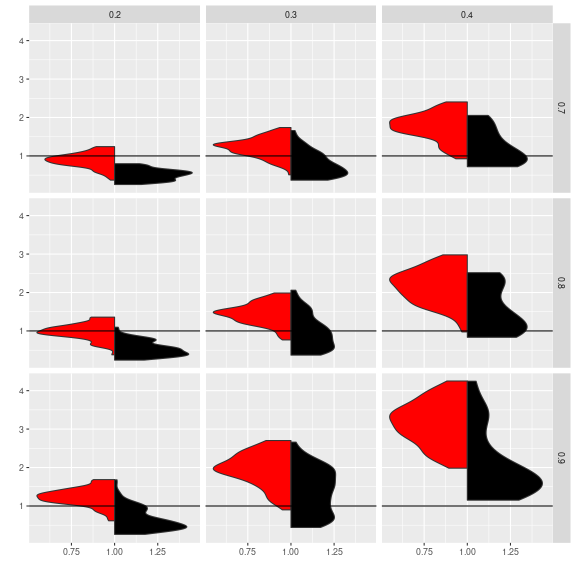
\includegraphics[width=\textwidth]{figures/v-b-1.png}
		\caption{$SSB/B_{MSY}$}
		\label{fig:grid-bmsy}
	\end{subfigure}
	\begin{subfigure}{0.32\textwidth}  
		\centering 
		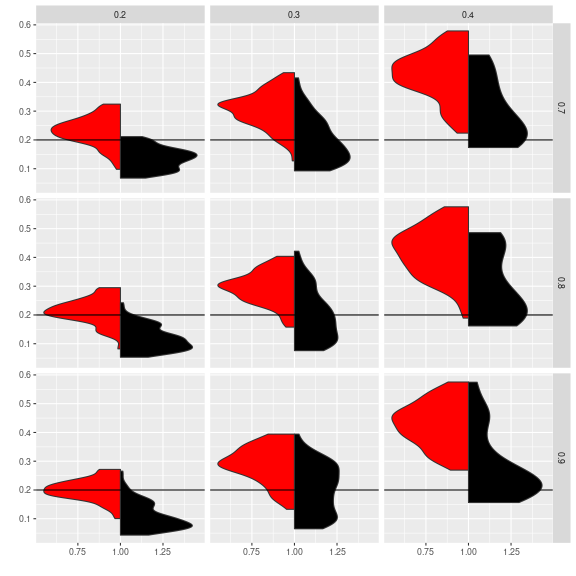
\includegraphics[width=\textwidth]{figures/v-m-1.png}
		\caption{$SSB/K$}
		\label{fig:grid-blim}
	\end{subfigure}
	\begin{subfigure}{0.32\textwidth}  
		\centering 
		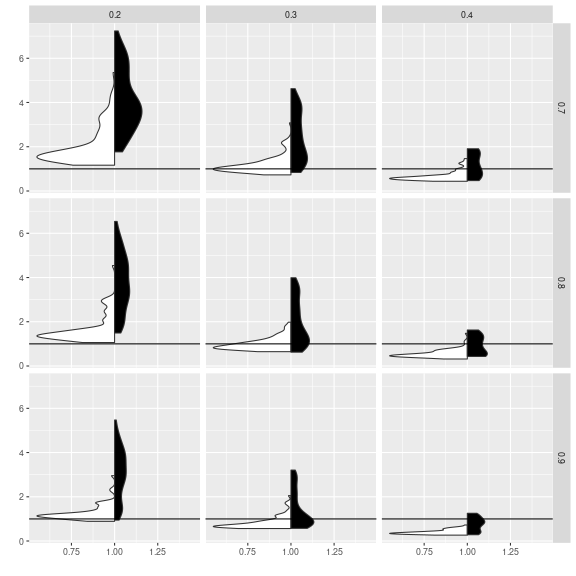
\includegraphics[width=\textwidth]{figures/v-h-1.png}
		\caption{$F/F_{MSY}$}
		\label{fig:grid-fmsy}
	\end{subfigure}
	\begin{subfigure}{0.32\textwidth}  
		\centering 
		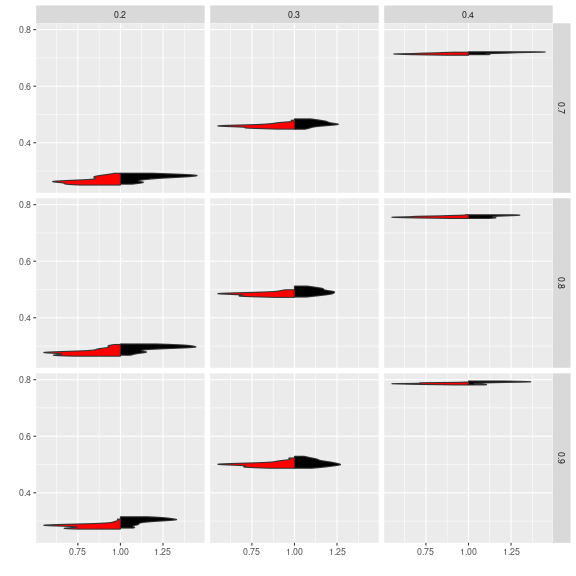
\includegraphics[width=\textwidth]{figures/v-r-1.png}
		\caption{$r$}
		\label{fig:grid-r}
	\end{subfigure}	\begin{subfigure}{0.32\textwidth}  
		\centering 
		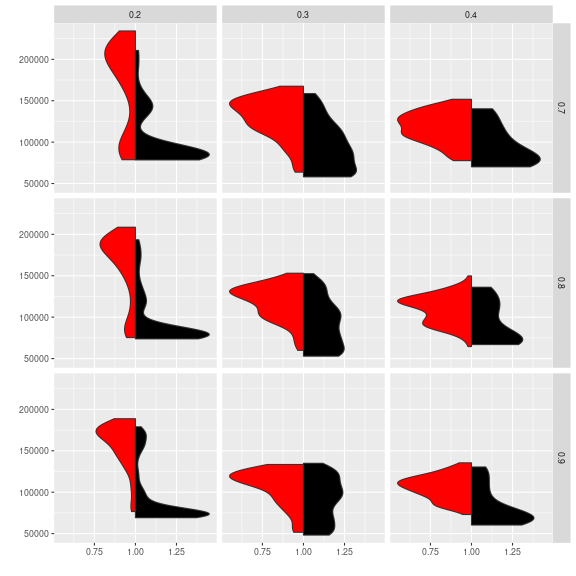
\includegraphics[width=\textwidth]{figures/v-k-1.png}
		\caption{$K$}
		\label{fig:grid-k}
	\end{subfigure}	\begin{subfigure}{0.32\textwidth}  
		\centering 
		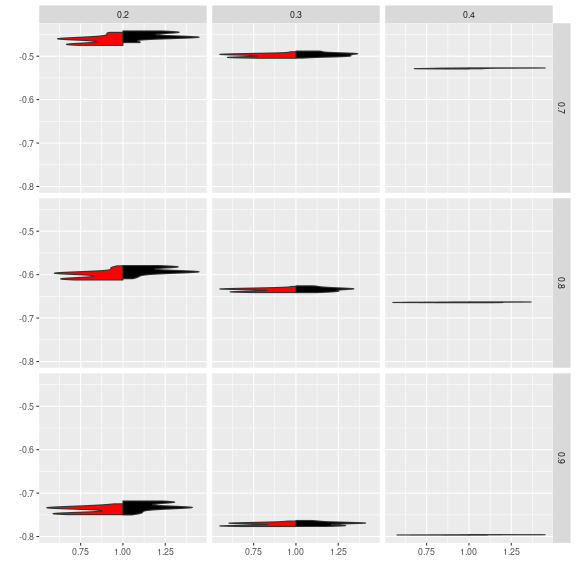
\includegraphics[width=\textwidth]{figures/v-p-1.png}
		\caption{$p$}
		\label{fig:grid-p}
	\end{subfigure}
	\begin{subfigure}{0.32\textwidth}  
		\centering 
		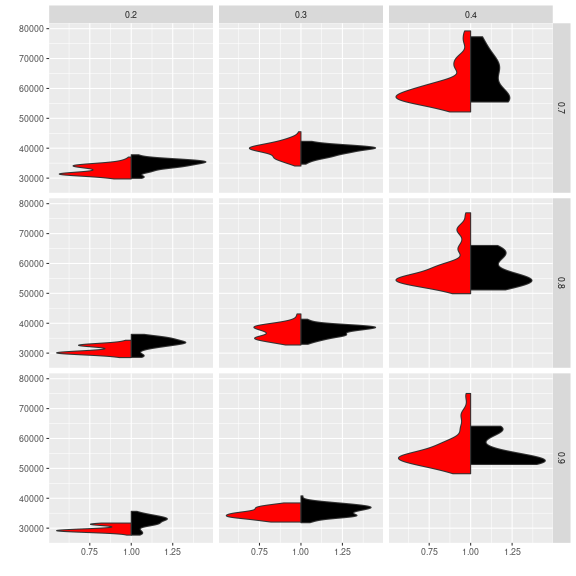
\includegraphics[width=\textwidth]{figures/v-sp-1.png}
		\caption{$sd(sp)$}
		\label{fig:grid-sp}
	\end{subfigure}	\begin{subfigure}{0.32\textwidth}  
		\centering 
		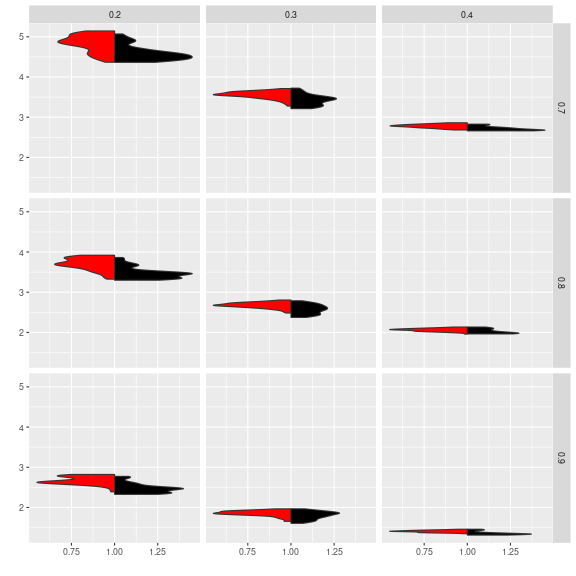
\includegraphics[width=\textwidth]{figures/v-d-1.png}
		\caption{Population doubling time}
		\label{fig:grid-dt}
	\end{subfigure}
	\caption{}
	\label{ref:grid}
\end{figure}

\iffalse
\begin{figure}[ht!]\centering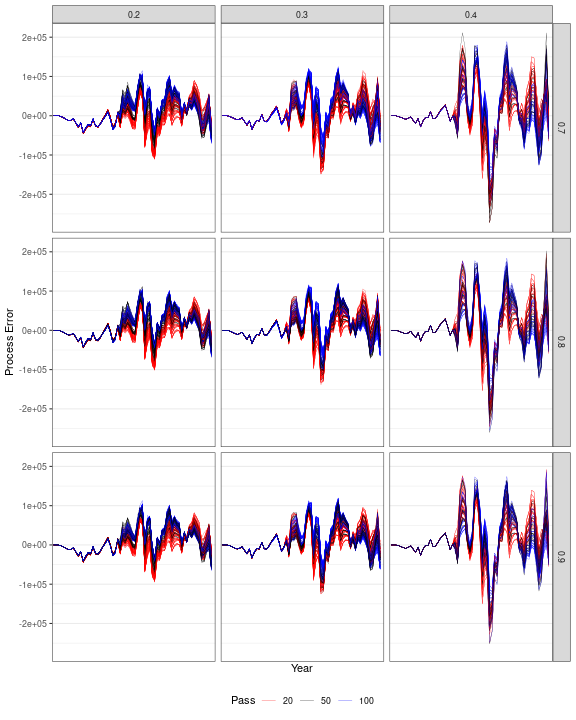
\includegraphics[width=0.75\textwidth]{figures/pf-1.png} 
\caption{Surplus Production by steepness and mature natural mortality}
\label{fig:sp}       
\end{figure}
\fi



\clearpage
\newpage
\section*{Weighting}

\begin{itemize}
    \item W(Expert): Expert opinion, assigned “a-priori”, without consideration of model fit.
    \item W(Convergence): Model convergence criteria of the estimation algorithm.
    \item W(Fit): The fit of the model to the data.
    \item W(Plausible parameters): The plausibility of the estimates of the parameters representing the
hypothesis.
    \item W(Plausible results): The plausibility of the model results.
    \item W(Diagnostics): Reliability of the model based on diagnostics.
\end{itemize}

\clearpage
\newpage
\newpage
\section*{Discussion}


When developing metrics as in any indicator, the total number should be minimised, complementary and non-redundant (Shin et al. 2010; Kershner et al. 2011). They should also be robust proxies for relevant attributes, and need to be screened using appropriate selection criteria \cite{kell2020roc}. To be effective a metric should be robust, so that it still functions despite uncertainty \parencite{radatz1990ieee, zhou1996robust}. To be robust an metric should be both reliable and stable. A metric has high reliability if despite uncertainty it provides an accurate result, and it is stable if despite random error, similar results are produced across multiple trials. 

\begin{itemize}
    \item The aim of this work was to evaluate the use of full factorial designs for representing uncertainty in stock assessment. In particular to identify the assumptions that impact the perception of stock dynamics and status, and develop tools for weighting or rejecting stock assessment scenarios.
  
    %\item The Indian Ocean Albacore MSE used Stock Synthesis to develop scenarios based on parameters that are difficult to estimate (i.e. M, steepness, and selectivity) and the relative weightings of the indices of abundance and the length data. The choice of OMs is important as the \textit{best} Management Procedure is determined by the choice of hypotheses represented by the OM. It seldom possible, however, to assign plausibility to the different scenarios, therefore the rationale for the grid design is of fundamental importance.

    %\item Need to consider the future not just the past
    
    \item The absence of retrospective patterns in model quantities such as stock biomass, is not sufficient to validate models based on model outputs, since a small RE could be achieved by a model that used no data.  Therefore conduct a hindcast.
    
    \item Can only validate models on observations and not model outputs, therefore need to conduct model free hindcasts to estimate prediction skill by comparing observations and to their model estimates, to explore bias, variability and prediction skill.
    
    \item Use the hindcast procedure to weight multi-model ensembles using simple skill-based weighting. A prediction skill score can be used to assign more weight on the better performing models as this has been found to improve forecasts \citep[e.g.][]{casanova2009weighting}. This can be done to weight estimates of current status relative to reference points, or weight operating models when conducting MSE. %Testing the approach on an actual case study first was informative as it provides the insight necessary to set up a study on synthetic data.

    %\item next step is assess prediction skill using model free hindcasting, as it allows comparisons to be made across model structures and datasets. Validation examines if a model family should be modified or extended and is complementary to model selection and hypothesis testing. In comparison model selection searches for the most suitable model within a family, whilst hypothesis testing examines if the model structure can be reduced. This is important as it allows alternative model frameworks to be compared and valiadated in a working group setting.

    %\item When conducting Management Strategy Evaluation (MSE) Operating Models (OMs) are commonly \citep{Sharma} conditioned using stock assessment models and a grid design to model structural uncertainty and data conflicts. However, there are two main characteristics of the stock dynamics i.e. the expected dynamics as represented by a production function and the nature of the times series. Therefore you could just run a limited number of scenarios that represent the different production functions an time series dynamics.

    \item \cite{fischer2020linking} showed that to develop robust management strategies the nature of the time series of the stock has to be considered. The importance of this is that trends and fluctuations in populations are determined by complex interactions between extrinsic forcing and intrinsic dynamics. For example, stochastic recruitment can induce low-frequency variability, i.e. ‘cohort resonance’, which can induce apparent trends in abundance and may be common in age-structured populations \citep[e.g.][]{bjoernstad2004trends, botsford2014cohort}. Such low-frequency fluctuations can mimic or cloak critical variation in abundance linked to environmental change, over-exploitation or other types of anthropogenic forcing. In feedback management systems the nature of the time series dynamics is likely to be more important than the equilibrium dynamics. 
    
    \item The objective of MSE is to develop a robust MP, so weighting of OM grids based on stock assessments is a waste of time. Since trends and fluctuations in populations are determined by complex interactions between extrinsic forcing and intrinsic dynamics. For example, stochastic recruitment can induce low-frequency variability, i.e. ‘cohort resonance’, which can induce apparent trends in abundance and may be common in age-structured populations \citep[e.g.][]{bjoernstad2004trends, botsford2014cohort}. Such low-frequency fluctuations can potentially mimic or cloak critical variation in abundance linked to environmental change, over-exploitation or other types of anthropogenic forcing. In feedback management systems the nature of the time series dynamics is likely to be more important than the equilibrium dynamics.

   \item Weighting give very different results wrt targets and limits, this is important, e.g. for MSC. Rather than arguing about the best weighting scheme better to develop robust MPs, that need to be tested for a range of plausible dynamics. 
   
\end{itemize} 



%\section{Conclusions}

I totally agree on the automation, to ensure objectively and transparency. Its like MSE where you have to agree the OMs and the MP selection criteria in advance.

Also like MSE, I think we need a limited number of complementary but non-redundant metrics. For example are the runs tests,  RMSE and Mohn's rho telling us the same thing? So we are give a single attribute extra weight? Imagine you have a model with a biased index, i.e. a data conflict, that fails the runs and RMSE tests. When you do retrospective you are removing biased points so you will get a large absolute value for Mohn's rho. In contrast MASE for a model free quantity will hopefully be telling you something else. It would be best to recognise that data conflict at the start.

For this reason I  agree with Mark that ideally a model should pass all diagnostics but recognise that this isn't always possible. For example if a model fails to converge that could indicate data conflicts and model misspecification, that will bite you later if not fixed. For example when you start removing points example in the retrospective analysis and hindcasts.

Also while the delta-MVLN approach is useful, I would also like to use estimation error to check bias, i.e. by looking at prediction residuals.

\begin{itemize}
    \item In the stock assessment process hypotheses about states of nature are represented by alternative model structures and fixed parameters. Even with a design of 1440, as in this example, the choice of scenarios is arbitrary and the posterior distributions are often multi-modal.
    
    \item Considering alternative structures and datasets means that it difficult to select models using metrics such as AIC. Therefore retrospective analysis is commonly used to evaluate the stability of stock assessment estimates.  The use of model based quantities, however, means that bias can not be quantified, and may result in future predictions being being poor. We therefore extended retrospective analyses to include predictions. 
   
    \item The use of metrics based on prediction skill allows different data components and model to be compared in order to explore data conflicts and potential model misspecification. The accuracy and precision of predictions depend on the validity of the model, the information in the data, and how far ahead predictions are required. 
   
    \item Retrospective analysis is commonly used to evaluate the stability of stock assessment estimates of model estimates such as stock biomass and exploitation level. Stability is measured using Mohn's $\rho$ a measure of bias. 
    
    \item Shrinking estimates of stock status in the last year to the recent mean can help reduce Mohn's $\rho$. Shrinkage, in statistics, however, is used to reduce mean squared error (MSE), at the expense of bias. 
    
    \item The use of model based quantities, however, means that bias can not be quantified, and may result in future predictions being being poor. We therefore extend retrospective analyses to include prediction. 

    \item When developing the design for ensembles or OMs first it is necessary to choose a base case, the main effects and interactions. A problem is that hypotheses are likely to be confounded e.g. i) is High M and low steepness realistic? ii) relative weighting of ESS and CPUE CV; and iii) dome shaped selection or senescence. If we had used the approach proposed would our conclusions have differed? Use of feedback relaxes requirement for prediction skill, ii) helps identify series for use in OEM, iii) what if OM scenarios have different "best" indices?

    %\item For models to be valid the situation being modelled must be observable and measurable. Therefore it is only possible to validate models on observations, the next step is to use model free hindcasting.
     
    %\item In order to develop robust advice frameworks by conducting Management Strategy Evaluation Operating Models should not be condition on stock assessments alone.

    %\item Hessian not inverting might be the most interesting result! i.e.  did we start from the wrong place, is there conflict or lack of information in the data, are the parameters confounded? is our structure wrong,... We need to answer these questions before we agree the ensemble.
    
    %\item The numerical tests may have different distributions and properties making using difficult to use for weighting, i.e. RMSE is influenced by a few outliers and is not comparable across series. While MASE  has the properties of scale invariance, predictable behaviour, symmetry, interpretability and asymptotic normality. MASE is also independent of the scale of the data, so can be used to compare forecasts across data sets with different scales, and behaviour is predictable as and a value of 0.5 means that a prediction is twice as good as one with a value of 1.
    
    %\item Tests have different purposes and different consequences, so equal weighting may be hard to justify. For example, if model residuals are fine, but prediction residuals fail. The consequences are  you may have overfitted, i.e. added too many parameters possibly as a result of hypothesis fishing, and the prediction residuals are telling you that your model is invalid, and so you need to start again.
    
    %\item  Bootstrapping depends on how the weights have been assigned and how the ensemble was selected.
\end{itemize}


\newpage\clearpage
\bibliographystyle{abbrvnat}
\bibliography{references.bib}

\end{document}

\clearpage
\newpage
\section{Tables}

\begin{table}[!ht]
\label{tab:grid}
\caption{Operating Model Scenarios; Base Case values in bold.}  
\begin{center}
\label{tab:datasumm}
\begin{tabular}{|lccc|}
\hline
& {\tiny Levels (N)} & {\tiny $\prod$ N} & {\tiny Values} \\ %& {\tiny Prior} & {\tiny Weighting}\\
\hline\hline
{\tiny Natural mortality (M)& {\tiny 5}}  & {\tiny   5}  & {\tiny  0202  \textbf{0303} 0404 0403 0402}    \\
{\tiny Steepness of the stock-recruitment relationship}}& {\tiny 3} 	 & {\tiny 15}  & {\tiny  \textbf{.7}; 0.8; 0.9} \\
{\tiny Variability of recruitment (sigmaR)}& {\tiny 2} 	 & {\tiny  30}  & {\tiny  \textbf{0.4}; 0.6} \\
{\tiny Effective Sampling Size of the length composition data (ESS)}& {\tiny 3} & {\tiny  90}  & {\tiny  20; \textbf{50}; 100} \\
{\tiny CV for fit to CPUE (cpuecv)}& {\tiny 2} 	 & {\tiny  360}  & {\tiny  0.2;  \textbf{0.3}; 0.4; 0.5} \\
{\tiny Yearly increase in catchability coefficient of CPUE (llq)}& {\tiny 2} 	 & {\tiny   720}  & {\tiny  \textbf{0\%}; 0.25\%} \\
{\tiny Selectivity (llsel)}& {\tiny 2}}& {\tiny 1440}} & {\tiny  \textbf{logistic} double normal} \\
\hline

\end{tabular}
\end{center}
\end{table}

\begin{table}[!ht]
\caption{Mohn's $\rho$ for retrospective analysis.}  
\label{tab:retro}
\centering
\begin{tabular}{rllr}
  \hline
 & run & variable & $\rho$ \\ 
  \hline
  1 & ... & stock & ... \\ 
   \hline
\end{tabular}
\end{table}


\end{document}

\subsection{How to include Figures}

First you have to upload the image file from your computer using the upload link the project menu. Then use the includegraphics command to include it in your document. Use the figure environment and the caption command to add a number and a caption to your figure. See the code for Figure \ref{fig:frog} in this section for an example.

\subsection{How to add Comments}

Comments can be added to your project by clicking on the comment icon in the toolbar above. % * <john.hammersley@gmail.com> 2016-07-03T09:54:16.211Z:
%
% Here's an example comment!
%
To reply to a comment, simply click the reply button in the lower right corner of the comment, and you can close them when you're done.

Comments can also be added to the margins of the compiled PDF using the todo command\todo{Here's a comment in the margin!}, as shown in the example on the right. You can also add inline comments:

\todo[inline, color=green!40]{This is an inline comment.}

\subsection{How to add Tables}

Use the table and tabular commands for basic tables --- see Table~\ref{tab:widgets}, for example. 

\begin{table}
\centering
\begin{tabular}{l|r}
Item & Quantity \\\hline
Widgets & 42 \\
Gadgets & 13
\end{tabular}
\caption{\label{tab:widgets}An example table.}
\end{table}

\subsection{How to write Mathematics}

\LaTeX{} is great at typesetting mathematics. Let $X_1, X_2, \ldots, X_n$ be a sequence of independent and identically distributed random variables with $\text{E}[X_i] = \mu$ and $\text{Var}[X_i] = \sigma^2 < \infty$, and let
\[S_n = \frac{X_1 + X_2 + \cdots + X_n}{n}
      = \frac{1}{n}\sum_{i}^{n} X_i\]
denote their mean. Then as $n$ approaches infinity, the random variables $\sqrt{n}(S_n - \mu)$ converge in distribution to a normal $\mathcal{N}(0, \sigma^2)$.


\subsection{How to create Sections and Subsections}

Use section and subsections to organize your document. Simply use the section and subsection buttons in the toolbar to create them, and we'll handle all the formatting and numbering automatically.

\subsection{How to add Lists}

You can make lists with automatic numbering \dots

\begin{enumerate}
\item Like this,
\item and like this.
\end{enumerate}
\dots or bullet points \dots
\begin{itemize}
\item Like this,
\item and like this.
\end{itemize}

\subsection{How to add Citations and a References List}

You can upload a \verb|.bib| file containing your BibTeX entries, created with JabRef; or import your \href{https://www.overleaf.com/blog/184}{Mendeley}, CiteULike or Zotero library as a \verb|.bib| file. You can then cite entries from it, like this: \cite{greenwade93}. Just remember to specify a bibliography style, as well as the filename of the \verb|.bib|.

You can find a \href{https://www.overleaf.com/help/97-how-to-include-a-bibliography-using-bibtex}{video tutorial here} to learn more about BibTeX.

We hope you find Overleaf useful, and please let us know if you have any feedback using the help menu above --- or use the contact form at \url{https://www.overleaf.com/contact}!